%Poster do trabalho de conclusao de curso 

\documentclass[final]{beamer}
\mode<presentation>{\usetheme{azul}}
\usepackage{graphicx}
\usepackage{epstopdf}
\usepackage{subfigure}

\usepackage[brazil]{babel}
\usepackage[utf8]{inputenc}
\usepackage{ragged2e} 


\usepackage{amsmath,amsthm, amssymb, latexsym}
\usepackage[orientation=portrait,size=a2,scale=1.4]{beamerposter}
\usepackage[ruled]{algorithm2e}

\usepackage{snapshot} % will write a .dep file with all dependencies, allows for easy bundling

\DeclareMathSizes{17.42}{15}{14}{10}  % Math text size

%%%%%%%%%%%%%%%%%%%%%%%%%%%%%%%%
%%  MACROS %%%%%%%%%%%%%%%%%%%%%
\usepackage{xspace}
\newcommand{\pixel}{\emph{pixel}\xspace}
\newcommand{\pixels}{\emph{pixels}\xspace}
\newcommand{\voxel}{\emph{voxel}\xspace}
\newcommand{\voxels}{\emph{voxels}\xspace}


\listfiles
%%%%%%%%%%%%%%%%%%%%%%%%%%%%%%%%%%%%%%%%%%%%%%%%%%%%%%%%%%%%%%%%%%%%%%%%%%%%%%%%%%%%%%
\title{\huge Atividade Curricular em Cultura e Extensão}

\author{Victor Sena Molero}
\institute[Universidade de São Paulo] % (optional, but mostly needed)
{
    Instituto de Matemática e Estatística, Universidade de São Paulo
}

\date{}
%%%%%%%%%%%%%%%%%%%%%%%%%%%%%%%%%%%%%%%%%%%%%%%%%%%%%%%%%%%%%%%%%%%%%%%%%%%%%%%%%%%%%%
\newlength{\columnheight}
\setlength{\columnheight}{65cm}
%%%%%%%%%%%%%%%%%%%%%%%%%%%%%%%%%%%%%%%%%%%%%%%%%%%%%%%%%%%%%%%%%%%%%%%%%%%%%%%%%%%%%%
\begin{document}
\begin{frame}
\begin{columns}
% ---------------------------------------------------------%
% Set up a column 
\begin{column}{.5\textwidth}
\begin{beamercolorbox}[center,wd=\textwidth]{postercolumn}
\begin{minipage}[T]{.95\textwidth} % tweaks the width, makes a new \textwidth
\parbox[t][\columnheight]{\textwidth}{ % must be some better way to set the the height, width and textwidth simultaneously
    \begin{block}{Introdução}
        O MaratonIME é um grupo de estudos da USP para competições de algoritmo, em especial para a Maratona de Programação, organizada pela Sociedade Brasileira de Computação, e que é classificatória para as finais mundiais da ACM-ICPC. Além disso, muitas outras competições deste tipo são feitas na internet e tem ampla participação de programadores de todo o mundo.
    \end{block}

    \begin{block}{Objetivos}
        O meu objetivo nesta matéria foi treinar minha habilidade como competidor de forma a me preparar para as várias fases da Maratona de Programação que vão ocorrer no semestre que vem. Para isso, me comprometi a cumprir as 100 horas exigidas pela matéria de MAC0214 como contests, ou seja, provas de competições de algoritmo, durante o semestre.
        \end{block}
    \begin{block}{Blog}
        \begin{figure}[h]
        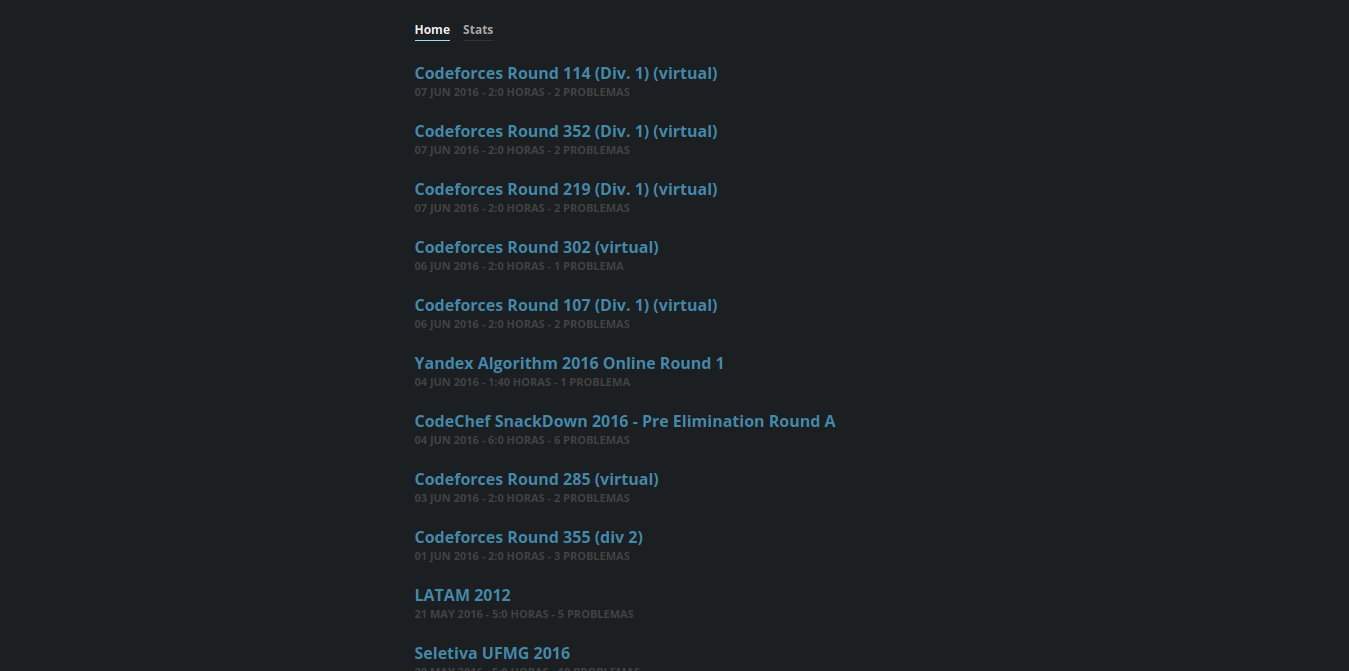
\includegraphics[scale=.40]{blog.png}
    \caption{Road do MAC0214}
    \end{figure}
    Durante o semestre eu registrei os contests que realizei num blog, para que meu progresso pudesse ser verificado. Ali são listados os problemas resolvidos durante o tempo de treino e os contests aos quais eles pertencem. O blog está disponível online em http://victorsenam.github.io/blog-mac0214
        \end{block}
    \begin{block}{Codeforces}
    \begin{figure}
    \centering
        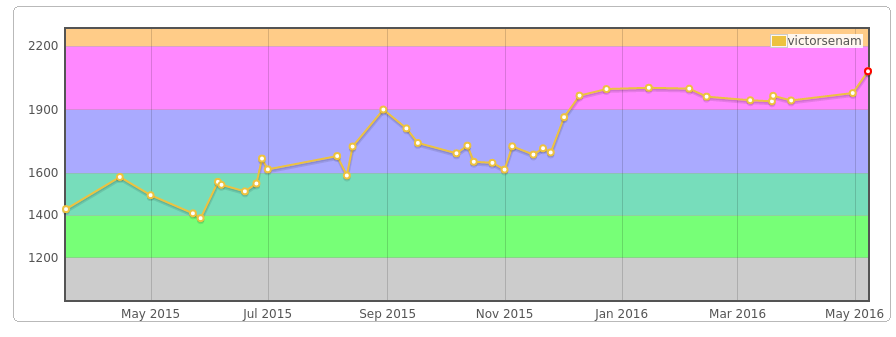
\includegraphics[width=0.95\textwidth]{codeforces.png}
    \caption{Meu perfil no Codeforces}
    \end{figure} 
    O Codeforces é um importante site voltado para programação competitiva. Grande parte dos meus treinos durante o semestre foram realizados neste site. Os contest são muito bem feitos e contam com problemas interessantes de diversos níveis.

        \end{block}

    \begin{block}{Perfis em Online Judges}
    \small
        \bibliographystyle{alpha} 
    \bibliography{ref}
    Codeforces - http://codeforces.com/profile/victorsenam \\
        TopCoder - https://www.topcoder.com/members/victorsenam/ \\
        Ahmed Aly - http://ahmed-aly.com/Profile.jsp?Username=victorsenam \\
        \end{block}
}
\end{minipage}
\end{beamercolorbox}
\end{column}
% ---------------------------------------------------------%
% end the column

% ---------------------------------------------------------%
% Set up a column 
\begin{column}{.5\textwidth}
\begin{beamercolorbox}[center,wd=\textwidth]{postercolumn}
\begin{minipage}[T]{.95\textwidth} % tweaks the width, makes a new \textwidth
\parbox[t][\columnheight]{\textwidth}{ % must be some better way to set the the height, width and textwidth simultaneously
    % Since all columns are the same length, it is all nice and tidy.  You have to get the height empirically
        % ---------------------------------------------------------%
        % fill each column with content

        \begin{block}{MaratonIME}
    \begin{figure}
    \centering
        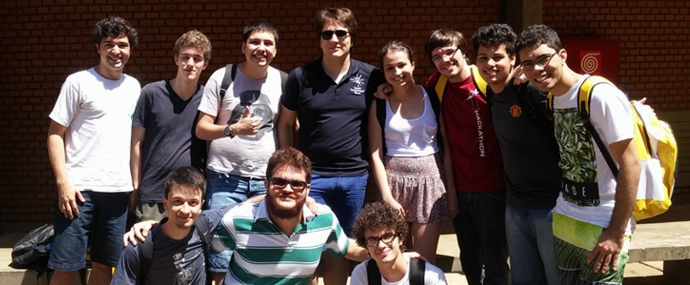
\includegraphics[width=0.95\textwidth]{maratonime.png}
    \caption{Grupo de estudos para a Maratona de Programação na Cidade Universitária}
    \end{figure} 
    O grupo de estudos MaratonIME reúne alunos interessados em treinar para competições de algoritmos. Durante o semestre algumas provas das quais eu participei foram organizadas pelo grupo.

        \end{block}
    \begin{block}{CodeChef Snackdown 2016}
        \begin{figure}[htp]
        \centering
        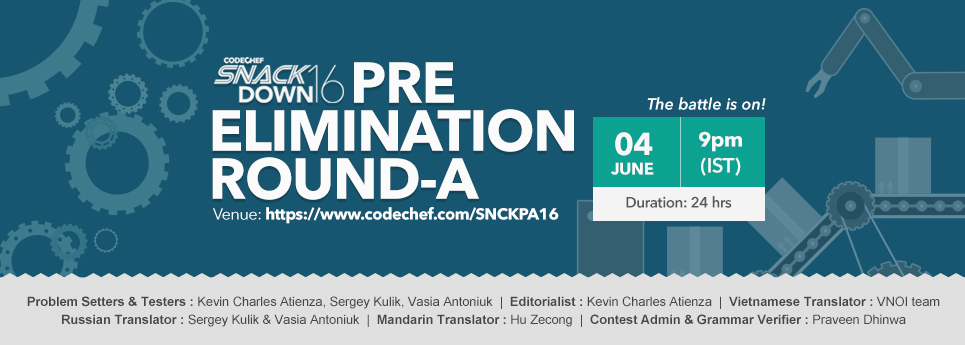
\includegraphics[width=0.95\textwidth]{snackdown.jpg}
    \caption{Divulgação do SnackDown 2016}
    \end{figure}
    No momento estou participando, em dupla com um outro aluno do IME, Gabriel de Russo e Carmo, da competição SnackDown 2016, organizada pelo CodeChef. Muitos alunos da USP estão participando e, neste ano, estamos classificados para a segunda fase online da competição. A fase classificatória foi cheia de problemas inteligentes e divertidos que abrangiam diversos tópicos de algoritmos e estruturas de dados.
        \end{block}
    \begin{block}{CodeJam 2016}
        \begin{figure}[htp]
        \centering
        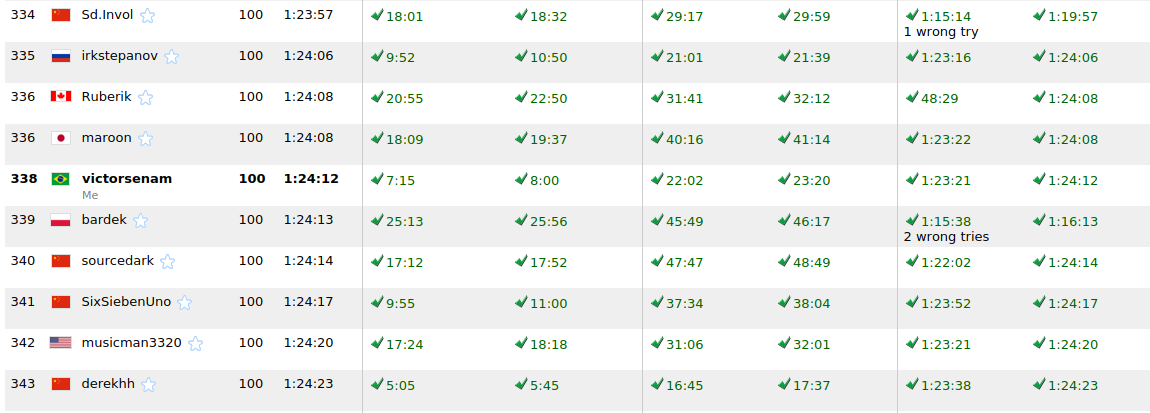
\includegraphics[width=0.95\textwidth]{codejam.png}
    \caption{Placar do Round 1A do CodeJam}
    \end{figure}
    Durante o semestre eu consegui me qualificar para o segundo round do Google CodeJam pela primeira vez atingindo a posição 338 no Round 1A e consegui atingir a posição 1129 durante o round 2. 
        \end{block}
    \begin{block}{Github e Upsolving}
    Todos os códigos submetidos nestes judges e de outros problemas que não foram submetidos durante contests estão disponíveis em um repositório público do github. A pasta onde eles estão pode ser acessada pelo seguinte link:  https://github.com/victorsenam/treinos/tree/master/victorsenam/ojs/ \\
        \end{block}
    \vfill
}
\end{minipage}
\end{beamercolorbox}
\end{column}
% ---------------------------------------------------------%
% end the column


\end{columns}
\end{frame}

\end{document}


%%%%%%%%%%%%%%%%%%%%%%%%%%%%%%%%%%%%%%%%%%%%%%%%%%%%%%%%%%%%%%%%%%%%%%%%%%%%%%%%%%%%%%%%%%%%%%%%%%%%
%%% Local Variables: 
%%% mode: latex
%%% TeX-PDF-mode: t
%%% End:
